\documentclass[11pt,a4paper]{article}

% --- Encoding and typography --------------------------------------------------
\usepackage[T1]{fontenc}
\usepackage[utf8]{inputenc}
\usepackage{lmodern}
\usepackage{microtype}

% --- Page geometry and running heads ------------------------------------------
\usepackage[margin=2.6cm,headheight=14pt]{geometry}
\usepackage{fancyhdr}
\pagestyle{fancy}
\fancyhf{}
\renewcommand{\headrulewidth}{0.4pt}
\fancyhead[L]{\footnotesize\scshape BiomedCAT Frontend}
\fancyhead[R]{\footnotesize\thepage}

% --- Sectioning ---------------------------------------------------------------
\usepackage{titlesec}
\titleformat{\section}{\normalfont\large\bfseries}{\thesection}{0.75em}{}
\titleformat{\subsection}{\normalfont\normalsize\bfseries}{\thesubsection}{0.75em}{}
\titlespacing*{\section}{0pt}{1.6em plus .3em minus .2em}{0.7em}
\titlespacing*{\subsection}{0pt}{1.1em plus .2em minus .2em}{0.5em}

% --- Floats and figures -------------------------------------------------------
\usepackage{tikz}
\usetikzlibrary{positioning, arrows.meta}
\usepackage[font=small,labelfont=bf,skip=8pt]{caption}

\usepackage[hidelinks]{hyperref}

% --- Document metadata --------------------------------------------------------
\newcommand{\docTitle}{BiomedCAT Frontend}
\newcommand{\docSubtitle}{Architecture and Developer Documentation}
\newcommand{\docAuthor}{Salah Eddine Chahma}
\newcommand{\docSupervisor}{Dr.\ Sandrine Muller}
\newcommand{\docTeam}{DAISY Team}
\newcommand{\docLab}{Laboratoire d'Informatique de Grenoble (LIG)}

\begin{document}
\thispagestyle{plain}

% --- Title block --------------------------------------------------------------
\begin{center}
  {\footnotesize\scshape \docLab\ \textperiodcentered\ \docTeam \par}

  \vspace{0.9em}
  \rule{\textwidth}{0.8pt}
  \vspace{0.55em}

  {\LARGE\bfseries \docTitle \par}
  \vspace{0.35em}
  {\large\itshape \docSubtitle \par}

  \vspace{0.55em}
  \rule{\textwidth}{0.4pt}

  \vspace{0.8em}
  {\normalsize \docAuthor \par}
  \vspace{0.2em}
  {\footnotesize Supervised by \docSupervisor \par}
  \vspace{0.5em}
  {\footnotesize \today \par}
\end{center}

\vspace{0.8em}

% ==============================================================================
\section{Introduction}

BiomedCAT extracts biomedical entities from presentation slides and grounds each
one in a public knowledge base. Processing proceeds in three stages: optical
character recognition transcribes the text of every slide, named entity
recognition identifies the biomedical terms and assigns each a type, and
normalisation resolves every term to a knowledge-base identifier. This document
specifies the web console through which those results are consulted, and is
intended for a reader who must maintain or extend it.

The console is an observation layer over a completed computation. It reads the
JSON files that the pipeline writes into the \texttt{Output} directory and
performs no inference of its own, a separation imposed by the cost of a run,
which requires a CUDA-capable GPU and several minutes per presentation. Submitting a presentation
through the interface copies it into the \texttt{Dataset} directory, from which
the pipeline collects it on its next invocation. Every quantity presented on
screen therefore refers to work that has already completed.

The interface comprises three views. \emph{Overview} enumerates the presentations
processed to date together with their aggregate totals, \emph{Run} presents a
single presentation in full, and \emph{About} documents the system for a non-technical
reader. Two application programming interface routes support them, one accepting
uploaded presentations and one serving an individual run as a JSON or CSV download. The
implementation uses Next.js 16.2.12, React 19.2.4, Tailwind CSS v4 and
TypeScript.

% ==============================================================================
\section{Software architecture}

\subsection{Layered organisation}

The source tree is partitioned by responsibility rather than by feature. Each of
the three directories under \texttt{src} answers a distinct question: from where
the displayed quantities originate, how they are rendered, and what each view
contains.

\begin{quote}
\begin{tabular}{@{}ll@{}}
\texttt{src/lib/}        & data access and derivation \\
\texttt{src/components/} & presentation \\
\texttt{src/app/}        & views and API routes \\
\end{tabular}
\end{quote}

Figure~\ref{fig:flow} traces a result from disk to the browser, and the reverse
path taken by a submitted presentation.

\begin{figure}[!ht]
\centering
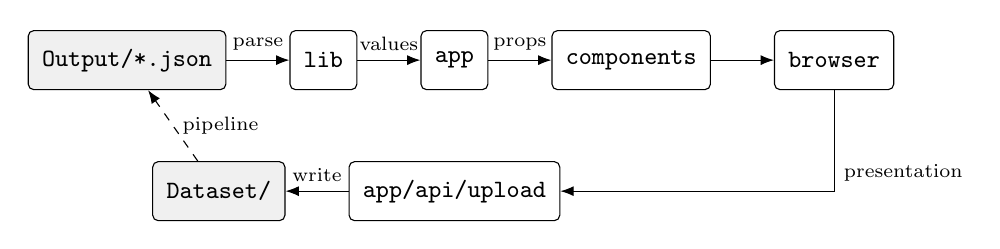
\begin{tikzpicture}[
  >=Latex,
  node distance=6mm and 8mm,
  box/.style={draw, rounded corners=2pt, minimum height=7.5mm,
              inner xsep=5pt, font=\small\ttfamily},
  store/.style={box, fill=black!6},
  lab/.style={font=\scriptsize, midway}
]
  \node[store] (out)  {Output/*.json};
  \node[box, right=of out]  (lib)  {lib};
  \node[box, right=of lib]  (app)  {app};
  \node[box, right=of app]  (comp) {components};
  \node[box, right=of comp] (br)   {browser};

  \draw[->] (out)  -- node[lab, above] {parse}  (lib);
  \draw[->] (lib)  -- node[lab, above] {values} (app);
  \draw[->] (app)  -- node[lab, above] {props}  (comp);
  \draw[->] (comp) -- (br);

  \node[box, below=9mm of app] (api) {app/api/upload};
  \node[store, left=of api] (ds) {Dataset/};

  \draw[->] (br) |- node[lab, above right] {presentation} (api);
  \draw[->] (api) -- node[lab, above] {write} (ds);
  \draw[->, dashed] (ds) -- node[lab, right] {pipeline} (out);
\end{tikzpicture}
\caption{Data flow through the console. The dashed transition is performed by the
processing pipeline, which executes outside the application.}
\label{fig:flow}
\end{figure}

\subsection{Module responsibilities}

\paragraph{Data access and derivation.}
The \texttt{lib} directory contains no presentation logic. \texttt{paths.ts}
resolves the location of the \texttt{Dataset} and \texttt{Output} directories;
\texttt{runs.ts} parses the result files into typed records and declares the
schema they are expected to satisfy; \texttt{queue.ts} compares the two
directories to determine which presentations remain unprocessed. Derived quantities are
computed in \texttt{stats.ts}, which aggregates entity counts and linking rates.
The remaining modules define presentation-independent vocabulary:
\texttt{entity-types.ts} fixes the seven entity types and their assigned colours,
\texttt{stages.ts} does likewise for the three pipeline stages, \texttt{decks.ts}
enumerates the accepted input formats, and \texttt{format.ts} together with
\texttt{csv.ts} converts values into displayed or exported text.

\paragraph{Presentation.}
The \texttt{components} directory holds the visual elements: cards, tables,
charts, badges, the navigation rail and the upload panel. Each receives finished
values as properties and determines only their appearance. No component reads
from disk or retrieves the data it displays; several import a type or a pure
helper from \texttt{lib}, for example to format a duration or to obtain the
colour of an entity type. The single component that communicates with the server
is the upload panel, which transmits a selected file to the upload route.
Excluding data acquisition from this layer is what permits a view to be
reorganised without modifying it.

\paragraph{Views and routes.}
Each view in \texttt{app} obtains what it requires from \texttt{lib} and composes
components around it. \texttt{page.tsx} implements the Overview,
\texttt{run/page.tsx} presents an individual presentation, \texttt{about/page.tsx}
provides the descriptive text, and \texttt{layout.tsx} defines the navigation and
frame common to all three. The two modules under \texttt{app/api} implement the
routes: the upload route writes an incoming presentation into \texttt{Dataset}, and the
export route returns a run as JSON or CSV. Colours, typefaces and type sizes are
declared once in \texttt{globals.css} and referenced by name throughout, so that
a change to a token propagates across the interface.

Dependencies are predominantly unidirectional. The \texttt{app} layer draws on
both others, \texttt{components} depend only on their properties and a small set
of pure helpers, and \texttt{lib} has no knowledge of the interface. A
modification to a computed quantity is therefore confined to \texttt{lib}, a
modification to its appearance to \texttt{components}, and a modification to the
composition of a view to \texttt{app}. File access is restricted to \texttt{lib}
and to the upload route, which is the only component of the system that writes.

\subsection{Execution model}

The Overview and Run views are regenerated on the server for every request, so
that a completed run becomes visible on reload without rebuilding or restarting
the application. The About view, whose content is static, is prerendered at build
time. Execution is otherwise confined to the server: only the navigation rail,
which marks the active view, and the upload panel, which handles file selection,
execute in the browser.

\subsection{Coupling with the processing pipeline}

The console and the pipeline share no code. Their coupling is established by two
conventions, both of which fail silently when violated. First, a presentation named
\texttt{FSHD1.pptx} must yield a result named \texttt{FSHD1\_BiomedCAT.json},
since the console reconstructs that name to determine which presentations remain
unprocessed. Second, the console does not validate a result against the schema it
declares, with the consequence that a renamed or retyped field produces an
incorrect value on screen rather than an error.

% ==============================================================================
\section{Installation and execution}

\subsection{Requirements}

The console requires Node.js 20.9 or later. It requires neither a GPU nor a
Python environment nor the model weights, as it reads only the artefacts the
pipeline has already produced.

\subsection{Development server}

From the \texttt{frontend} directory, dependencies are installed once and the
development server started:

\begin{quote}
\ttfamily
cd FinalVersion/frontend \\
npm install \\
npm run dev
\end{quote}

\noindent The console is then served at \texttt{http://localhost:3000}.

\subsection{Directory resolution}

The \texttt{Dataset} and \texttt{Output} directories are expected to reside
alongside the \texttt{frontend} directory, which is the standard repository
layout. Where this does not hold, the \texttt{BIOMEDCAT\_ROOT} environment
variable specifies the directory that contains them:

\begin{quote}
\ttfamily
BIOMEDCAT\_ROOT=/path/to/FinalVersion npm run dev
\end{quote}

\noindent Neither directory is required to exist in advance. In their absence the
views render normally and report that no runs were found, which is the expected
state prior to the first execution of the pipeline.

\subsection{Production build}

A production build is produced with \texttt{npm run build} and served with
\texttt{npm start}.

\end{document}